\setlength{\pdfpagewidth}{210mm}
\setlength{\pdfpageheight}{297mm}
\documentclass[journal, transmag]{IEEEtran}
\hyphenation{op-tical net-works semi-conduc-tor}
\usepackage{hyperref,color,breqn,multirow}
\usepackage[top=0.7in, left=0.65in]{geometry}
\usepackage{graphicx}
\setlength{\textwidth}{7.2in}
\setlength{\textheight}{9.6in}

\setlength{\tabcolsep}{4pt}

% additional packages
\usepackage{siunitx}
\usepackage{float}
\usepackage{subcaption}
\usepackage{amsmath}
\usepackage{amssymb}

% \usepackage{tikz}
% \usepackage{pgfplots}
% \pgfplotsset{compat=newest}
% \usepackage{pgfplotstable}
% \usepackage{tuda-pgfplots}
%
% \usetikzlibrary{external}
% \tikzexternalize

\begin{document}
    \title{Shape Optimization of a Photo-Electron Gun\\ using Isogeometric Analysis}

    \author{\IEEEauthorblockN{Peter Förster\IEEEauthorrefmark{1}, Sebastian Schöps\IEEEauthorrefmark{1}, Joachim Enders\IEEEauthorrefmark{2}, Maximilian Herbert\IEEEauthorrefmark{2} and Abele Simona\IEEEauthorrefmark{3}} \IEEEauthorblockA{\IEEEauthorrefmark{1}Institute for Accelerator Science and Electromagnetic Fields, Technische Universität Darmstadt, Germany} \IEEEauthorblockA{\IEEEauthorrefmark{2}Institut für Kernphysik, Fachbereich Physik, Technische Universität Darmstadt, Germany} \IEEEauthorblockA{\IEEEauthorrefmark{3}Laboratory for Modeling and Scientific Computing, Politecnico Milano, Italy}}

    \IEEEtitleabstractindextext{
    \begin{abstract}
        A key design problem for photo-electron guns is minimizing the electric field strength on the electrode surface to avoid field emission. Isogeometric analysis (IGA) allows to compute accurate approximations of the field by using non-uniform rational B-splines (NURBS) to describe both the computational domain and the numerical solution. The control points of these NURBS offer an intuitive set of degrees of freedom, and make it possible to freeform optimize the shape of the electrode efficiently. Several beam parameters are considered in the optimization to ensure proper gun performance. The results of an IGA-based shape optimization for a planned high-voltage upgrade of the photogun teststand Photo-CATCH at TU Darmstadt are presented.
    \end{abstract}

    \begin{IEEEkeywords}
        Design optimization, Electron guns, Finite element analysis, Particle tracking, Splines (mathematics)
    \end{IEEEkeywords}}

    \maketitle
    \thispagestyle{empty}
    \pagestyle{empty}

    \section{Introduction}
    \IEEEPARstart{T}{he design} of high-voltage dc photo-electron guns deals with two major difficulties: The optimization of beam parameters depending on the planned application, and the minimization of field emission. The first issue has been at the center of much research for a long time, see, e.g., \cite{pierce1940}, \cite{radley1958}. However, field emission may still have a detrimental effect on the beam parameters, and it can even severely damage gun components. To avoid this, the electric field strength on the surface of the electrode needs to be minimized. Since the field strongly depends on the geometry of the electrode, numerical shape optimization may be used to solve this problem.

    Previous approaches commonly employed parameter optimization to this end, compare \cite{bazarov2005}. In contrast, we freeform shape optimize the geometry using non-uniform rational B-splines (NURBS) \cite{piegl1997}, a technique that reduces manual effort and still allows precise control over the solution space via refinement strategies such as knot insertion and degree elevation.

    NURBS also form the basis of isogeometric analysis (IGA) \cite{cottrell2009}, thus it is natural to use IGA for the numerical solution of the field problem. Moreover, using higher order NURBS basis functions leads to a higher global regularity of the solution compared to classical finite element approaches. This can represent a meaningful advantage, especially when performing particle tracking simulations.

    The new workflow is applied to the photo-electron gun at TU Darmstadt's Photo-Cathode Activation, Test, and Cleaning (Photo-CATCH) facility \cite{kurichiyanil2019}, where an upgrade from \SIrange{-60}{-300}{\kilo\volt} bias voltage is planned.

    \section{Mathematical Formulation}
    Linear combinations of basis functions $N_{i,p}$ of a NURBS space may be used to define NURBS curves
    \begin{align*}
        C_{\mathbf{P}}(\xi) = \sum_i \mathbf{P}_i N_{i,p}(\xi),
    \end{align*}
    where $p$ denotes the degree of the underlying B-spline basis, and the coefficients $\mathbf{P} \subset \mathbb{R}^3$ are called control points. Changes in the positions of these control points smoothly influence the shape of the curve, thus they form an intuitive and easily accessable set of degrees of freedom for numerical shape optimization. A tensor product construction gives NURBS volumes, which are patched together such that they describe the overall domain $\boldsymbol{\Omega}(\mathbf{P})$, compare \cite{buffa2015}. We use the NURBS package \cite{spink2017} for the computational handling of the geometries.

    \begin{figure}
        \begin{center}
        % \begin{tikzpicture}
\begin{axis}[
    scale only axis=true,
    width=0.5\textwidth,
    axis equal,
    enlargelimits=true,
    colormap={bg}{color=(TUDa-1a) color=(TUDa-3a)},
    point meta min=1,
    point meta max=2,
    legend columns=4,
    legend style={at={(0.06, 0.8)}, anchor=north west, draw=none, fill=none},
    hide axis]

    % legend
    \addplot[color=TUDa-5a, very thick] table{dat/boundary_orig14.dat};
    \addlegendentry{$\boldsymbol{\Gamma}_{\mathrm{D}_0}$};
    \addplot[color=TUDa-7a, densely dashed, very thick] table{dat/boundary_orig63.dat};
    \addlegendentry{$\boldsymbol{\Gamma}_{\mathrm{D}_1}$};
    \addplot[color=TUDa-9a, densely dotted, very thick] table{dat/boundary_orig32.dat};
    \addlegendentry{$\boldsymbol{\Gamma}_{\mathrm{D}_2}$};
    \addplot[color=black, very thick] table{dat/boundary_orig11.dat};
    \addlegendentry{Symmetry axis};

    \addplot[surf, shader=interp, area legend, fill=TUDa-1a] table[point meta=\thisrow{c}]{dat/geometry5.dat};
    \addlegendentry{$\boldsymbol{\Omega}_{\mathrm{ins}}^{\mathrm{2D}}$};
    \addplot[surf, shader=interp, area legend, fill=TUDa-3a] table[point meta=\thisrow{c}*2]{dat/geometry14.dat};
    \addlegendentry{$\boldsymbol{\Omega}_{\mathrm{opt}}^{\mathrm{2D}}$};

    % insulator
    \addplot[surf, shader=interp] table[point meta=\thisrow{c}]{dat/geometry23.dat};
    \addplot[surf, shader=interp] table[point meta=\thisrow{c}]{dat/geometry24.dat};
    \addplot[surf, shader=interp] table[point meta=\thisrow{c}]{dat/geometry31.dat};
    \addplot[surf, shader=interp] table[point meta=\thisrow{c}]{dat/geometry32.dat};
    \addplot[surf, shader=interp] table[point meta=\thisrow{c}]{dat/geometry33.dat};
    \addplot[surf, shader=interp] table[point meta=\thisrow{c}]{dat/geometry34.dat};

    % optimization
    \addplot[surf, shader=interp] table[point meta=\thisrow{c}*2]{dat/geometry15.dat};
    \addplot[surf, shader=interp] table[point meta=\thisrow{c}*2]{dat/geometry16.dat};
    \addplot[surf, shader=interp] table[point meta=\thisrow{c}*2]{dat/geometry17.dat};
    \addplot[surf, shader=interp] table[point meta=\thisrow{c}*2]{dat/geometry18.dat};

    % patch boundaries
    \addplot[color=TUDa-0d, thin] table{dat/boundary_orig13.dat};
    \addplot[color=TUDa-0d, thin] table{dat/boundary_orig22.dat};
    \addplot[color=TUDa-0d, thin] table{dat/boundary_orig23.dat};
    \addplot[color=TUDa-0d, thin] table{dat/boundary_orig33.dat};
    \addplot[color=TUDa-0d, thin] table{dat/boundary_orig43.dat};
    \addplot[color=TUDa-0d, thin] table{dat/boundary_orig52.dat};
    \addplot[color=TUDa-0d, thin] table{dat/boundary_orig62.dat};
    \addplot[color=TUDa-0d, thin] table{dat/boundary_orig72.dat};
    \addplot[color=TUDa-0d, thin] table{dat/boundary_orig82.dat};
    \addplot[color=TUDa-0d, thin] table{dat/boundary_orig92.dat};
    \addplot[color=TUDa-0d, thin] table{dat/boundary_orig102.dat};
    \addplot[color=TUDa-0d, thin] table{dat/boundary_orig113.dat};
    \addplot[color=TUDa-0d, thin] table{dat/boundary_orig123.dat};
    \addplot[color=TUDa-0d, thin] table{dat/boundary_orig133.dat};
    \addplot[color=TUDa-0d, thin] table{dat/boundary_orig142.dat};
    \addplot[color=TUDa-0d, thin] table{dat/boundary_orig153.dat};
    \addplot[color=TUDa-0d, thin] table{dat/boundary_orig163.dat};
    \addplot[color=TUDa-0d, thin] table{dat/boundary_orig171.dat};
    \addplot[color=TUDa-0d, thin] table{dat/boundary_orig173.dat};
    \addplot[color=TUDa-0d, thin] table{dat/boundary_orig183.dat};
    \addplot[color=TUDa-0d, thin] table{dat/boundary_orig191.dat};
    \addplot[color=TUDa-0d, thin] table{dat/boundary_orig193.dat};
    \addplot[color=TUDa-0d, thin] table{dat/boundary_orig201.dat};
    \addplot[color=TUDa-0d, thin] table{dat/boundary_orig211.dat};
    \addplot[color=TUDa-0d, thin] table{dat/boundary_orig213.dat};
    \addplot[color=TUDa-0d, thin] table{dat/boundary_orig221.dat};
    \addplot[color=TUDa-0d, thin] table{dat/boundary_orig231.dat};
    \addplot[color=TUDa-0d, thin] table{dat/boundary_orig233.dat};
    \addplot[color=TUDa-0d, thin] table{dat/boundary_orig241.dat};
    \addplot[color=TUDa-0d, thin] table{dat/boundary_orig251.dat};
    \addplot[color=TUDa-0d, thin] table{dat/boundary_orig254.dat};
    \addplot[color=TUDa-0d, thin] table{dat/boundary_orig261.dat};
    \addplot[color=TUDa-0d, thin] table{dat/boundary_orig264.dat};
    \addplot[color=TUDa-0d, thin] table{dat/boundary_orig271.dat};
    \addplot[color=TUDa-0d, thin] table{dat/boundary_orig274.dat};
    \addplot[color=TUDa-0d, thin] table{dat/boundary_orig281.dat};
    \addplot[color=TUDa-0d, thin] table{dat/boundary_orig291.dat};
    \addplot[color=TUDa-0d, thin] table{dat/boundary_orig303.dat};
    \addplot[color=TUDa-0d, thin] table{dat/boundary_orig313.dat};
    \addplot[color=TUDa-0d, thin] table{dat/boundary_orig323.dat};
    \addplot[color=TUDa-0d, thin] table{dat/boundary_orig333.dat};

    % vacuum chamber
    \addplot[color=TUDa-5a, very thick] table{dat/boundary_orig12.dat};
    \addplot[color=TUDa-5a, very thick] table{dat/boundary_orig54.dat};
    \addplot[color=TUDa-5a, very thick] table{dat/boundary_orig111.dat};
    \addplot[color=TUDa-5a, very thick] table{dat/boundary_orig112.dat};
    \addplot[color=TUDa-5a, very thick] table{dat/boundary_orig114.dat};
    \addplot[color=TUDa-5a, very thick] table{dat/boundary_orig122.dat};
    \addplot[color=TUDa-5a, very thick] table{dat/boundary_orig132.dat};
    \addplot[color=TUDa-5a, very thick] table{dat/boundary_orig152.dat};
    \addplot[color=TUDa-5a, very thick] table{dat/boundary_orig162.dat};
    \addplot[color=TUDa-5a, very thick] table{dat/boundary_orig192.dat};
    \addplot[color=TUDa-5a, very thick] table{dat/boundary_orig202.dat};
    \addplot[color=TUDa-5a, very thick] table{dat/boundary_orig203.dat};
    \addplot[color=TUDa-5a, very thick] table{dat/boundary_orig223.dat};
    \addplot[color=TUDa-5a, very thick] table{dat/boundary_orig243.dat};
    \addplot[color=TUDa-5a, very thick] table{dat/boundary_orig253.dat};
    \addplot[color=TUDa-5a, very thick] table{dat/boundary_orig343.dat};

    % neumann
    \addplot[color=black, very thick] table{dat/boundary_orig21.dat};
    \addplot[color=black, very thick] table{dat/boundary_orig31.dat};
    \addplot[color=black, very thick] table{dat/boundary_orig41.dat};
    \addplot[color=black, very thick] table{dat/boundary_orig61.dat};
    \addplot[color=black, very thick] table{dat/boundary_orig311.dat};
    \addplot[color=black, very thick] table{dat/boundary_orig321.dat};
    \addplot[color=black, very thick] table{dat/boundary_orig331.dat};
    \addplot[color=black, very thick] table{dat/boundary_orig341.dat};

    % anode ring
    \addplot[color=TUDa-9a, densely dotted, very thick] table{dat/boundary_orig42.dat};
    \addplot[color=TUDa-9a, densely dotted, very thick] table{dat/boundary_orig74.dat};
    \addplot[color=TUDa-9a, densely dotted, very thick] table{dat/boundary_orig84.dat};
    \addplot[color=TUDa-9a, densely dotted, very thick] table{dat/boundary_orig94.dat};
    \addplot[color=TUDa-9a, densely dotted, very thick] table{dat/boundary_orig104.dat};
    \addplot[color=TUDa-9a, densely dotted, very thick] table{dat/boundary_orig131.dat};
    \addplot[color=TUDa-9a, densely dotted, very thick] table{dat/boundary_orig53.dat};

    % electrode
    \addplot[color=TUDa-7a, densely dashed, very thick] table{dat/boundary_orig73.dat};
    \addplot[color=TUDa-7a, densely dashed, very thick] table{dat/boundary_orig83.dat};
    \addplot[color=TUDa-7a, densely dashed, very thick] table{dat/boundary_orig93.dat};
    \addplot[color=TUDa-7a, densely dashed, very thick] table{dat/boundary_orig103.dat};
    \addplot[color=TUDa-7a, densely dashed, very thick] table{dat/boundary_orig143.dat};
    \addplot[color=TUDa-7a, densely dashed, very thick] table{dat/boundary_orig151.dat};
    \addplot[color=TUDa-7a, densely dashed, very thick] table{dat/boundary_orig161.dat};
    \addplot[color=TUDa-7a, densely dashed, very thick] table{dat/boundary_orig174.dat};
    \addplot[color=TUDa-7a, densely dashed, very thick] table{dat/boundary_orig184.dat};
    \addplot[color=TUDa-7a, densely dashed, very thick] table{dat/boundary_orig181.dat};
    \addplot[color=TUDa-7a, densely dashed, very thick] table{dat/boundary_orig234.dat};
    \addplot[color=TUDa-7a, densely dashed, very thick] table{dat/boundary_orig272.dat};
    \addplot[color=TUDa-7a, densely dashed, very thick] table{dat/boundary_orig283.dat};
    \addplot[color=TUDa-7a, densely dashed, very thick] table{dat/boundary_orig282.dat};
    \addplot[color=TUDa-7a, densely dashed, very thick] table{dat/boundary_orig284.dat};
    \addplot[color=TUDa-7a, densely dashed, very thick] table{dat/boundary_orig294.dat};
    \addplot[color=TUDa-7a, densely dashed, very thick] table{dat/boundary_orig304.dat};
    \addplot[color=TUDa-7a, densely dashed, very thick] table{dat/boundary_orig301.dat};
    \addplot[color=TUDa-7a, densely dashed, very thick] table{dat/boundary_orig314.dat};
\end{axis}

    % coordinate axes
    \draw[->, >=latex, thick] (0.3, 2.2) to (0.8, 2.2);
    \node[right] at (0.8, 2.2) {$z$};
    \draw[->, >=latex, thick] (0.3, 2.2) to (0.3, 2.7);
    \node[above] at (0.3, 2.7) {$\rho$};
\end{tikzpicture}

        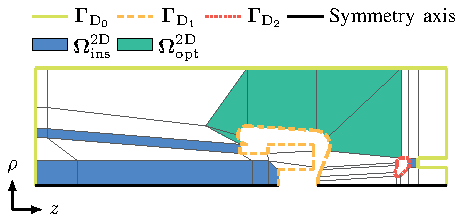
\includegraphics[width=0.45\textwidth]{geometry_original}
        \caption{Original geometry and boundary conditions of the computational domain $\boldsymbol{\Omega}^{\mathrm{2D}}$. Grey lines indicate patch boundaries.}
        \label{fig:geometry_original}
        \end{center}
    \end{figure}

    \subsection{Isogeometric Analysis}
    We look at the electrostatic approximation to Maxwell's equations, described by the following boundary value problem
    \begin{align*}
        \nabla \cdot \Big( \varepsilon \nabla \phi(\mathbf{x}) \Big) = 0 \quad \mathbf{x} \in \boldsymbol{\Omega}, \quad \varepsilon(\mathbf{x}) =
        \begin{cases}
            \begin{alignedat}{2}
                &\varepsilon_{\mathrm{ins}} &\quad &\mathbf{x} \in \boldsymbol{\Omega}_{\mathrm{ins}}\\
                &\varepsilon_0 &\quad &\text{otherwise},
            \end{alignedat}
        \end{cases}
    \end{align*}
    where $\phi$ is the electrostatic potential, and $\varepsilon_{\mathrm{ins}}$, $\varepsilon_0$ are the permittivity of the insulator and empty space respectively. The boundaries associated with the vacuum chamber $\boldsymbol{\Gamma}_{\mathrm{D}_0}$, electrode $\boldsymbol{\Gamma}_{\mathrm{D}_1}$, and anode ring $\boldsymbol{\Gamma}_{\mathrm{D}_2}$ are indicated in \autoref{fig:geometry_original}. For the computational domain $\boldsymbol{\Omega}^{\mathrm{2D}}$, we only consider half of a cross section of $\boldsymbol{\Omega}$, due to the axisymmetry of the geometry.

    Using a finite-dimensional approximation of the weak form of the electrostatic problem allows to express the potential as $\phi_h = \sum_i \varphi_i v_i, \varphi_i \in \mathbb{R}$, where the basis functions $v_i$ are chosen from a NURBS space according to the isogeometric setting. The discrete potential is then obtained by solving a linear system of equations
    \begin{align*}
        \mathbf{K}_\varepsilon \boldsymbol{\varphi} = - \boldsymbol{\rho}, \quad [\mathbf{K}_\varepsilon]_{ij} = \int_{\boldsymbol{\Omega}^{\mathrm{2D}}} \varepsilon \nabla v_j \cdot \nabla v_i\: \rho\: \mathrm{d}\rho\: \mathrm{d}z,
    \end{align*}
    and the approximated electric field follows from $\mathbf{E}_h = - \nabla \phi_h$. For the implementation of IGA we employ GeoPDEs \cite{vazquez2016}.

    \subsection{Particle Tracking}
    In a second step, the discrete field $\mathbf{E}_h$ may be used to perform particle simulations. These aim to solve the particles' equations of motion
    \begin{align*}
        \frac{\mathrm{d}\mathbf{x}}{\mathrm{d}t} = \mathbf{v} \quad \text{and} \quad \frac{\mathrm{d}\mathbf{p}}{\mathrm{d}t} = q (\mathbf{E}_h + \mathbf{v} \times \mathbf{B}_h),
    \end{align*}
    where $\mathbf{x}$, $\mathbf{v}$, $\mathbf{p}$ denote the position, velocity, and momentum of a given particle, and $\mathbf{B}_h$ is the magnetic field. Statistical beam parameters such as the rms beam widths and length, and the related transverse and longitudinal emittances can be extracted from the tracking results and incorporated into the optimization procedure. This allows to specify constraints on these quantities, in order to achieve a high quality beam with the optimized design.

    \begin{figure}[b]
        \begin{center}
        % \begin{tikzpicture}
\begin{axis}[
   scale only axis = true,
   width = 0.45\textwidth,
   axis equal,
   try min ticks=4,
   max space between ticks=1000pt,
   enlargelimits=true,
   x unit=m,
   y unit=m]

   \addplot[color=brewergrey] table {figures/200kV/nurbs/nurbs_5_1.dat};
   \addplot[color=brewerred, mark=*] table {figures/200kV/nurbs/nurbs_5_1_coefs.dat};
   \addplot[color=brewergrey, dashed] table {figures/200kV/nurbs/nurbs_5_1_net.dat};

   \addplot[color=brewergrey] table {figures/200kV/nurbs/nurbs_6_3.dat};
   \addplot[color=brewerred, mark=*] table {figures/200kV/nurbs/nurbs_6_3_coefs.dat};
   \addplot[color=brewergrey, dashed] table {figures/200kV/nurbs/nurbs_6_3_net.dat};

   \addplot[color=brewergrey] table {figures/200kV/nurbs/nurbs_7_3.dat};
   \addplot[color=brewerred, mark=*] table {figures/200kV/nurbs/nurbs_7_3_coefs.dat};
   \addplot[color=brewergrey, dashed] table {figures/200kV/nurbs/nurbs_7_3_net.dat};

   \addplot[color=brewergrey] table {figures/200kV/nurbs/nurbs_8_3.dat};
   \addplot[color=brewerred, mark=*] table {figures/200kV/nurbs/nurbs_8_3_coefs.dat};
   \addplot[color=brewergrey, dashed] table {figures/200kV/nurbs/nurbs_8_3_net.dat};

   \addplot[color=brewergrey] table {figures/200kV/nurbs/nurbs_9_3.dat};
   \addplot[color=brewerred, mark=*] table {figures/200kV/nurbs/nurbs_9_3_coefs.dat};
   \addplot[color=brewergrey, dashed] table {figures/200kV/nurbs/nurbs_9_3_net.dat};

   \addplot[color=brewergrey] table {figures/200kV/nurbs/nurbs_10_2.dat};
   \addplot[color=brewerred, mark=*] table {figures/200kV/nurbs/nurbs_10_2_coefs.dat};
   \addplot[color=brewergrey, dashed] table {figures/200kV/nurbs/nurbs_10_2_net.dat};

   \addplot[color=brewergrey] table {figures/200kV/nurbs/nurbs_11_2.dat};
   \addplot[color=brewerred, mark=*] table {figures/200kV/nurbs/nurbs_11_2_coefs.dat};
   \addplot[color=brewergrey, dashed] table {figures/200kV/nurbs/nurbs_11_2_net.dat};
\end{axis}
\end{tikzpicture}

        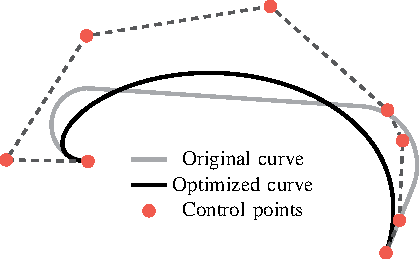
\includegraphics[width=0.4\textwidth]{nurbs}
        \caption{Original and optimized curves (including the optimized control points) describing the critical part of the electrode.}
        \label{fig:nurbs}
        \end{center}
    \end{figure}

    \subsection{Shape Optimization}
    We only optimize the shape of the critical part of the electrode, given by that part of $\boldsymbol{\Gamma}_{\mathrm{D}_1}$, which intersects with $\boldsymbol{\Omega}_{\mathrm{opt}}^{\mathrm{2D}}$, see \autoref{fig:nurbs}. The restriction to $\boldsymbol{\Omega}_{\mathrm{opt}}^{\mathrm{2D}}$ is motivated by the observation that the largest field magnitudes occur in this region, compare \autoref{fig:field}.

    We include constraints on the volume of the electrode $V_{\mathrm{e}}(\mathbf{P})$, given by the domain circumscribed by (revolving) $\boldsymbol{\Gamma}_{\mathrm{D}_1}$, and on the beam parameters obtained from the particle simulations $\mathbf{f}_{\mathrm{p}}(\mathbf{E}_h)$. Only allowing geometries from an admissible set $\mathcal{A}$, that contains additional constraints on the control points $\mathbf{P}$ to ensure manufacturability, we state the optimization problem as follows
    \begin{align*}
        \begin{cases}
            \begin{alignedat}{2}
                &\min_{\mathbf{P} \in \mathcal{A}} &\max_{\mathbf{x} \in \boldsymbol{\Omega}_{\mathrm{opt}}^{\mathrm{2D}}(\mathbf{P})} &\| \mathbf{E}_h(\mathbf{x}; \mathbf{P}) \|_2\\
                &\quad \mathrm{s.t.} &\mathbf{E}_h(\mathbf{x}; \mathbf{P}) &= - \nabla \phi_h(\mathbf{x}; \mathbf{P})\\
                &\quad &V_{\mathrm{e}}(\mathbf{P}) &\leq V_c\\
                &\quad &\mathbf{f}_{\mathrm{p}} \Big( \mathbf{E}_h(\mathbf{x}; \mathbf{P}) \Big) &< \mathbf{c},
            \end{alignedat}
        \end{cases}
    \end{align*}
    where $V_c$ is the maximum allowable volume, and $\mathbf{c}$ is a vector of real numbers constraining the individual beam parameters. The problem is solved numerically using algorithms from the NLopt nonlinear-optimization package \cite{johnson2020}.

    \begin{figure}[t]
        \begin{center}
        \begin{subfigure}{0.45\textwidth}
            \begin{center}
            % \begin{tikzpicture}
\begin{axis}[
    scale only axis=true,
    width=\textwidth,
    axis equal,
    enlargelimits=true,
    colormap name=tuda,
    point meta min=0,
    point meta max=13,
    hide axis]

    \addplot[surf, shader=faceted] table[point meta=\thisrow{c}*1e-6]{dat/E_orig_degree=3_nsub=16_npts=9_1.dat};
    \addplot[surf, shader=faceted] table[point meta=\thisrow{c}*1e-6]{dat/E_orig_degree=3_nsub=16_npts=9_2.dat};
    \addplot[surf, shader=faceted] table[point meta=\thisrow{c}*1e-6]{dat/E_orig_degree=3_nsub=16_npts=9_3.dat};
    \addplot[surf, shader=faceted] table[point meta=\thisrow{c}*1e-6]{dat/E_orig_degree=3_nsub=16_npts=9_4.dat};
    \addplot[surf, shader=faceted] table[point meta=\thisrow{c}*1e-6]{dat/E_orig_degree=3_nsub=16_npts=9_5.dat};
    \addplot[surf, shader=faceted] table[point meta=\thisrow{c}*1e-6]{dat/E_orig_degree=3_nsub=16_npts=9_6.dat};
    \addplot[surf, shader=faceted] table[point meta=\thisrow{c}*1e-6]{dat/E_orig_degree=3_nsub=16_npts=9_7.dat};
    \addplot[surf, shader=faceted] table[point meta=\thisrow{c}*1e-6]{dat/E_orig_degree=3_nsub=16_npts=9_8.dat};
    \addplot[surf, shader=faceted] table[point meta=\thisrow{c}*1e-6]{dat/E_orig_degree=3_nsub=16_npts=9_9.dat};
    \addplot[surf, shader=faceted] table[point meta=\thisrow{c}*1e-6]{dat/E_orig_degree=3_nsub=16_npts=9_10.dat};
    \addplot[surf, shader=faceted] table[point meta=\thisrow{c}*1e-6]{dat/E_orig_degree=3_nsub=16_npts=9_11.dat};
    \addplot[surf, shader=faceted] table[point meta=\thisrow{c}*1e-6]{dat/E_orig_degree=3_nsub=16_npts=9_12.dat};
    \addplot[surf, shader=faceted] table[point meta=\thisrow{c}*1e-6]{dat/E_orig_degree=3_nsub=16_npts=9_13.dat};
    \addplot[surf, shader=faceted] table[point meta=\thisrow{c}*1e-6]{dat/E_orig_degree=3_nsub=16_npts=9_14.dat};
    \addplot[surf, shader=faceted] table[point meta=\thisrow{c}*1e-6]{dat/E_orig_degree=3_nsub=16_npts=9_15.dat};
    \addplot[surf, shader=faceted] table[point meta=\thisrow{c}*1e-6]{dat/E_orig_degree=3_nsub=16_npts=9_16.dat};
    \addplot[surf, shader=faceted] table[point meta=\thisrow{c}*1e-6]{dat/E_orig_degree=3_nsub=16_npts=9_17.dat};
    \addplot[surf, shader=faceted] table[point meta=\thisrow{c}*1e-6]{dat/E_orig_degree=3_nsub=16_npts=9_18.dat};
    \addplot[surf, shader=faceted] table[point meta=\thisrow{c}*1e-6]{dat/E_orig_degree=3_nsub=16_npts=9_19.dat};
    \addplot[surf, shader=faceted] table[point meta=\thisrow{c}*1e-6]{dat/E_orig_degree=3_nsub=16_npts=9_20.dat};
    \addplot[surf, shader=faceted] table[point meta=\thisrow{c}*1e-6]{dat/E_orig_degree=3_nsub=16_npts=9_21.dat};
    \addplot[surf, shader=faceted] table[point meta=\thisrow{c}*1e-6]{dat/E_orig_degree=3_nsub=16_npts=9_22.dat};
    \addplot[surf, shader=faceted] table[point meta=\thisrow{c}*1e-6]{dat/E_orig_degree=3_nsub=16_npts=9_23.dat};
    \addplot[surf, shader=faceted] table[point meta=\thisrow{c}*1e-6]{dat/E_orig_degree=3_nsub=16_npts=9_24.dat};
    \addplot[surf, shader=faceted] table[point meta=\thisrow{c}*1e-6]{dat/E_orig_degree=3_nsub=16_npts=9_25.dat};
    \addplot[surf, shader=faceted] table[point meta=\thisrow{c}*1e-6]{dat/E_orig_degree=3_nsub=16_npts=9_26.dat};
    \addplot[surf, shader=faceted] table[point meta=\thisrow{c}*1e-6]{dat/E_orig_degree=3_nsub=16_npts=9_27.dat};
    \addplot[surf, shader=faceted] table[point meta=\thisrow{c}*1e-6]{dat/E_orig_degree=3_nsub=16_npts=9_28.dat};
    \addplot[surf, shader=faceted] table[point meta=\thisrow{c}*1e-6]{dat/E_orig_degree=3_nsub=16_npts=9_29.dat};
    \addplot[surf, shader=faceted] table[point meta=\thisrow{c}*1e-6]{dat/E_orig_degree=3_nsub=16_npts=9_30.dat};
    \addplot[surf, shader=faceted] table[point meta=\thisrow{c}*1e-6]{dat/E_orig_degree=3_nsub=16_npts=9_31.dat};
    \addplot[surf, shader=faceted] table[point meta=\thisrow{c}*1e-6]{dat/E_orig_degree=3_nsub=16_npts=9_32.dat};
    \addplot[surf, shader=faceted] table[point meta=\thisrow{c}*1e-6]{dat/E_orig_degree=3_nsub=16_npts=9_33.dat};
    \addplot[surf, shader=faceted] table[point meta=\thisrow{c}*1e-6]{dat/E_orig_degree=3_nsub=16_npts=9_34.dat};
\end{axis}
\end{tikzpicture}

            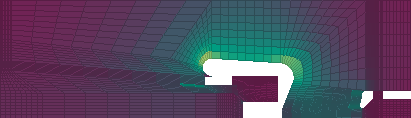
\includegraphics[width=\textwidth]{field_original}
            \end{center}
        \end{subfigure}

        \medskip

        \begin{subfigure}{0.45\textwidth}
            \begin{center}
            % \begin{tikzpicture}
\begin{axis}[
    scale only axis=true,
    width=\textwidth,
    axis equal,
    enlargelimits=true,
    colormap name=tuda,
    point meta min=0,
    point meta max=13,
    hide axis]

    \addplot[surf, shader=faceted] table[point meta=\thisrow{c}*1e-6]{dat/E_degree=3_nsub=16_npts=9_1.dat};
    \addplot[surf, shader=faceted] table[point meta=\thisrow{c}*1e-6]{dat/E_degree=3_nsub=16_npts=9_2.dat};
    \addplot[surf, shader=faceted] table[point meta=\thisrow{c}*1e-6]{dat/E_degree=3_nsub=16_npts=9_3.dat};
    \addplot[surf, shader=faceted] table[point meta=\thisrow{c}*1e-6]{dat/E_degree=3_nsub=16_npts=9_4.dat};
    \addplot[surf, shader=faceted] table[point meta=\thisrow{c}*1e-6]{dat/E_degree=3_nsub=16_npts=9_5.dat};
    \addplot[surf, shader=faceted] table[point meta=\thisrow{c}*1e-6]{dat/E_degree=3_nsub=16_npts=9_6.dat};
    \addplot[surf, shader=faceted] table[point meta=\thisrow{c}*1e-6]{dat/E_degree=3_nsub=16_npts=9_7.dat};
    \addplot[surf, shader=faceted] table[point meta=\thisrow{c}*1e-6]{dat/E_degree=3_nsub=16_npts=9_8.dat};
    \addplot[surf, shader=faceted] table[point meta=\thisrow{c}*1e-6]{dat/E_degree=3_nsub=16_npts=9_9.dat};
    \addplot[surf, shader=faceted] table[point meta=\thisrow{c}*1e-6]{dat/E_degree=3_nsub=16_npts=9_10.dat};
    \addplot[surf, shader=faceted] table[point meta=\thisrow{c}*1e-6]{dat/E_degree=3_nsub=16_npts=9_11.dat};
    \addplot[surf, shader=faceted] table[point meta=\thisrow{c}*1e-6]{dat/E_degree=3_nsub=16_npts=9_12.dat};
    \addplot[surf, shader=faceted] table[point meta=\thisrow{c}*1e-6]{dat/E_degree=3_nsub=16_npts=9_13.dat};
    \addplot[surf, shader=faceted] table[point meta=\thisrow{c}*1e-6]{dat/E_degree=3_nsub=16_npts=9_14.dat};
    \addplot[surf, shader=faceted] table[point meta=\thisrow{c}*1e-6]{dat/E_degree=3_nsub=16_npts=9_15.dat};
    \addplot[surf, shader=faceted] table[point meta=\thisrow{c}*1e-6]{dat/E_degree=3_nsub=16_npts=9_16.dat};
    \addplot[surf, shader=faceted] table[point meta=\thisrow{c}*1e-6]{dat/E_degree=3_nsub=16_npts=9_17.dat};
    \addplot[surf, shader=faceted] table[point meta=\thisrow{c}*1e-6]{dat/E_degree=3_nsub=16_npts=9_18.dat};
    \addplot[surf, shader=faceted] table[point meta=\thisrow{c}*1e-6]{dat/E_degree=3_nsub=16_npts=9_19.dat};
    \addplot[surf, shader=faceted] table[point meta=\thisrow{c}*1e-6]{dat/E_degree=3_nsub=16_npts=9_20.dat};
    \addplot[surf, shader=faceted] table[point meta=\thisrow{c}*1e-6]{dat/E_degree=3_nsub=16_npts=9_21.dat};
    \addplot[surf, shader=faceted] table[point meta=\thisrow{c}*1e-6]{dat/E_degree=3_nsub=16_npts=9_22.dat};
    \addplot[surf, shader=faceted] table[point meta=\thisrow{c}*1e-6]{dat/E_degree=3_nsub=16_npts=9_23.dat};
    \addplot[surf, shader=faceted] table[point meta=\thisrow{c}*1e-6]{dat/E_degree=3_nsub=16_npts=9_24.dat};
    \addplot[surf, shader=faceted] table[point meta=\thisrow{c}*1e-6]{dat/E_degree=3_nsub=16_npts=9_25.dat};
    \addplot[surf, shader=faceted] table[point meta=\thisrow{c}*1e-6]{dat/E_degree=3_nsub=16_npts=9_26.dat};
    \addplot[surf, shader=faceted] table[point meta=\thisrow{c}*1e-6]{dat/E_degree=3_nsub=16_npts=9_27.dat};
    \addplot[surf, shader=faceted] table[point meta=\thisrow{c}*1e-6]{dat/E_degree=3_nsub=16_npts=9_28.dat};
    \addplot[surf, shader=faceted] table[point meta=\thisrow{c}*1e-6]{dat/E_degree=3_nsub=16_npts=9_29.dat};
    \addplot[surf, shader=faceted] table[point meta=\thisrow{c}*1e-6]{dat/E_degree=3_nsub=16_npts=9_30.dat};
    \addplot[surf, shader=faceted] table[point meta=\thisrow{c}*1e-6]{dat/E_degree=3_nsub=16_npts=9_31.dat};
    \addplot[surf, shader=faceted] table[point meta=\thisrow{c}*1e-6]{dat/E_degree=3_nsub=16_npts=9_32.dat};
    \addplot[surf, shader=faceted] table[point meta=\thisrow{c}*1e-6]{dat/E_degree=3_nsub=16_npts=9_33.dat};
    \addplot[surf, shader=faceted] table[point meta=\thisrow{c}*1e-6]{dat/E_degree=3_nsub=16_npts=9_34.dat};
\end{axis}
\end{tikzpicture}

            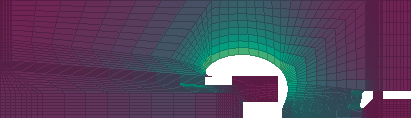
\includegraphics[width=\textwidth]{field_optimized}
            \end{center}
        \end{subfigure}
        \begin{subfigure}{\textwidth}
            \begin{center}
            % \begin{tikzpicture}
\begin{axis}[
    scale only axis=true,
    width=0.5\textwidth,
    axis equal,
    try min ticks=4,
    max space between ticks=1000pt,
    enlargelimits=true,
    colormap name=tuda,
    point meta min=0,
    point meta max=13,
    colorbar horizontal,
    colorbar style={xshift=-1.35*\pgfkeysvalueof{/pgfplots/parent axis width}, width=0.75*\pgfkeysvalueof{/pgfplots/parent axis width},
    xlabel=$\| \mathbf{E}_h \|_2$ (\si{\mega\volt\per\meter})},
    hide axis]

    \addplot[draw=none] coordinates{(0,0)};
\end{axis}
\end{tikzpicture}

            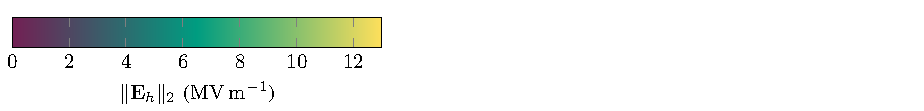
\includegraphics[width=0.9\textwidth]{colorbar}
            \end{center}
        \end{subfigure}
        \caption{Electric field magnitude for the original (top) and optimized (bottom) geometries. Computed using GeoPDEs.}
        \label{fig:field}
        \end{center}
    \end{figure}

    \section{Numerical Results}
    Preliminary optimization results can be seen in \autoref{fig:field}. The maximum absolute field strength visibly decreases, from \SI{13}{\mega\volt\per\meter} down to around \SI{9}{\mega\volt\per\meter}. This constitutes a reduction of almost \SI{25}{\percent}, illustrating the effectiveness of the approach. Furthermore, the optimized geometry adheres to all constraints, and the smooth shape is manufacturable. The full paper will include the shapes of the right side of the electrode $\boldsymbol{\Gamma}_{\mathrm{D}_1}$ and the anode ring $\boldsymbol{\Gamma}_{\mathrm{D}_2}$ into the optimization. These parts of the geometry greatly influence the beam parameters, thus we will also present corresponding particle tracking results.

\begin{thebibliography}{1}
    \bibitem{pierce1940}
    J.~R.~Pierce, ``Rectilinear electron flow in beams,'' \emph{J. Appl. Phys.,} vol. 11, pp. 548-554, 1940.

    \bibitem{radley1958}
    D.~E.~Radley, ``The theory of the Pierce type electron gun,'' \emph{J. Electron. Control,} vol. 4, pp. 125-148, 1958.

    \bibitem{bazarov2005}
    I.~V.~Bazarov and C.~K.~Sinclair, ``Multivariate optimization of a high brightness dc gun photoinjector,'' \emph{Phys. Rev. ST Accel. Beams,} vol. 8, 2005.

    \bibitem{piegl1997}
    L.~Piegl and W.~Tiller, ``The NURBS book,'' 1997.

    \bibitem{cottrell2009}
    J.~A.~Cottrell, T.~J.~R.~Hughes and Y.~Bazilevs, ``Isogeometric analysis: toward integration of CAD and FEA,'' 2009.

    \bibitem{kurichiyanil2019}
    N.~Kurichiyanil, J.~Enders, Y.~Fritzsche and M.~Wagner, ``A test system for optimizing quantum efficiency and dark lifetime of GaAs photocathodes,'' \emph{J. Instrum.,} vol. 14, 2019.

    \bibitem{buffa2015}
    A.~Buffa, R.~H.~Vázquez, G.~Sangalli and L.~B.~a.~da Veiga, ``Approximation estimates for isogeometric spaces in multipatch geometries,'' \emph{Numer. Methods Partial Differ. Equ.}, vol. 31, 2015.

    \bibitem{spink2017}
    M.~Spink, D.~Claxton, C.~de Falco and R.~Vázquez, ``NURBS package,'' 2017.

    \bibitem{vazquez2016}
    R.~Vázquez, ``A new design for the implementation of isogeometric analysis in Octave and Matlab: GeoPDEs 3.0,'' \emph{Comput. Math. Appl.,} vol. 72, 2016.

    \bibitem{johnson2020}
    S.~G.~Johnson, ``The NLopt nonlinear-optimization package,'' 2020.

    % \bibitem{boor2001}
    % C.~de Boor, ``A practical guide to splines,'' \emph{Appl. Math. Sci.,} vol. 27, 2001.

    % additional
    % \bibitem{powell1994}
    % M.~J.~D.~Powell, ``A direct search optimization method that models the objective and constraint functions by linear interpolation,'' \emph{Advances in Optimization and Numerical Analysis,} pp. 51–67, 1994.

    % \bibitem{jackson1998}
    % J.~D.~Jackson, ``Classical electrodynamics,'' 1998.

    % \bibitem{monk2003}
    % P.~Monk, ``Finite element methods for Maxwell’s equations,'' 2003.
\end{thebibliography}

\end{document}
